\section{Introduction}
\subsection{Motivation and Background}
Since the Fortran 2008 standard (published in 2010~\cite{iso2010fortran}), Fortran supports a \gls{spmd} programming style
that facilitates the creation of a fixed number of replicas of a compiled program that execute asynchronously after a program
initiation.  Fortran refers to each replica as an image.  The primary mechanism for distributing and communicating data between
images involves defining \glspl{coarray}, an entity that may be referenced or defined on one image by statements executing on
other images. As such, a coarray defines a \gls{pgas}.

The seminal role that \gls{coarray} played in the development of Fortran's intrinsic parallel programming model have made it
common to refer to all of Fortran's parallel programming features under the rubric of ``\gls{caf}.''  To date, most applications
of \gls{caf} involve applications where the parallelization itself poses one of the chief challenges and custom parallel
parallel algorithms must be developed~\cite{preissl2011multithreaded,garain2015comparing,mozdzynski2015partitioned}.  In such settings, the moniker \gls{caf} seems appropriate as much of the parallel programming effort centers around expressing the algorithm in \gls{coarray} syntax.

Less widely appreciated is the role that Fortran may play in embarassingly parallel applications for which the upcoming
Fortran 2015 standard (to be published in 2018\footnote{A Committee Draft is at https://bit.ly/fortran-2015-draft.}) will
will provide several useful features.  These include the ability to declare teams of images that communicate with each other
by default and collective subroutines that enable compiler and parallel runtime library developers to offer highly optimized
implementations of common communication patterns such as broadcasts and reductions.

Fortran 2015 might well meet the parallel algorithmic needs of embarassingly parallel applications without the need to declare
any \glspl{coarray}.  A common use case will involve conducting an ensemble of simulations, each of which executes in a separate
image team and with any communication occuring in the collective subroutines provided by the new standard.  This paper presents
such a use case for a terrestrial hydrological model developed at \gls{ncar}: the \gls{wrf-hydro}.  For this work, we wrote
what we believe is the first implementation of compiler support for teams.  In addition to providing an open-source capability
for studying the teams features defined in the draft Fortran 2015 standard, our implementation offers a language extension
that is intended to facilitate the incremental introductionof \gls{caf} in an already functioning \gls{mpi} application.

\subsection{Objectives}

\section{Methodology}
\subsection{Teams implementation in GNU Fortran}
\subsection{Teams support in OpenCoarrays}
\subsection{Teams use in WRF-Hydro}

WRF-Hydro is a community hydrologic modeling system developed at the
National Center for Atmospheric Research.  WRF-Hydro provides a
parallel-computing framework for coupling Numerical Weather Prediction models, land surface models, and a suite of hydrologic routing modules that handle
spatial water redistribution via surface (overland) flow,
subsurface (soil column) flow, baseflow (deep groundwater), and stream
channel transport~\cite{gochisEtal}. 

While originally developed to couple land hydrology to the atmospheric processes of
the WRF model, WRF-Hydro is most commonly run in ``offline'' mode where it is one-way
coupled to (forced by) prescribed upper boundary (weather)
conditions. The chief example is NOAA's operational
National Water Model~\cite{noaa2016}; a special configuration of
WRF-Hydro which provides real-time analysis and forecasts of
hydrologic states over the contiguous U.S. 

Ensemble forecasting and ensemble data assimilation are active and
growing areas of research with WRF-Hydro. Running ensembles under a
single executable and job submission on HPC platforms can greatly reduce the amount
of labor involved in designing workflows and can open up new
possibilities for improving data flows and optimizing ensemble run
performance.

In the application of teams to WRF Hydro, the main WRF-Hydro program is wrapped in a loop
over the individual ensemble members. The number of images per team and the
 number of ensemble members are specified in a namelist. Along  with
 the number of available images, these parameters determine how many
 teams are formed and which teams handle which ensemble members. It is
 worth noting several details of separate runs which may potentially need altering
 when running enembles via teams: 1) MPIINIT, 2) MPIFINALIZE, 3)
 variable initialization and allocation, 4) STOP.   
 

\section{Discussion of Results}

\section{Conclusions}

\section{Introduction to Teams}\label{sec:teams}
The existing coarray definition in Fortran 2008 does not provide for an environment
where a subset of the images can easily work on part of an application without affecting
other images in the program.  Grouping the images of a program into nonoverlapping
teams allows one to execute more effectively and independently parts of a larger
problem.  A class of problems that can benefit from this feature is multiphysics codes
(e.g.  climate models).
Such a feature, called \textit{Teams} in the Fortran 2015 standard, can significantly reduce the amount of off-node
communication on an exascale machine, in particular when an entire team of images
fits within a single compute node.
So far, the only compiler with a partial support for this new feature is the GNU Fortran Compiler (from now on
called GFortran) and a special version of the OpenCoarrays library.
In this Section we are going to introduce the basic constructs of \textit{Teams} and how OpenCoarrays implements them.

A team of images is a set of images that can readily execute independently of other images.
Initially, the current team consists of all images and this is
known as the initial team. Except for the initial team, every team has a unique parent team. A team is divided
into new teams by executing a \texttt{FORM TEAM} statement.
Each new team is identified by an integer value known
as its team number. Information about the team to which the current image belongs can be determined by the
processor from the collective value of the team variables on the images of the team.
The \texttt{FORM TEAM} statement is a collective operation executed by all the images.

During execution, each image has a current team, which is only changed by execution of \texttt{CHANGE TEAM} and
\texttt{END TEAM} statements. Executing a \texttt{CHANGE TEAM} statement changes the current team to the team specified
by the team-variable, and execution of the corresponding \texttt{END TEAM} statement restores the current team back
to that immediately prior to execution of the \texttt{CHANGE TEAM} statement.

Teams are described by a scalar variable called \texttt{TEAM TYPE}. This variable is a derived type with private components.
The \texttt{FORM TEAM} statement takes as first argument a team number that uniquely identifies the team and a \texttt{TEAM TYPE}
variable as second argument.
Successful execution of a \texttt{FORM TEAM} statement assigns the team-variable (of type \texttt{TEAM TYPE}) on each
participating image a value that specifies the new team that the image will belong to.
The \texttt{CHANGE TEAM} statement takes as argument a \texttt{TEAM TYPE} variable that represents the new team to be used as
current team. The execution of the \texttt{END TEAM} statement restores the current team back
to that immediately prior to execution of the \texttt{CHANGE TEAM} statement.

\subsection{Teams implementation}\label{subsec:teams_implementation}

From an MPI perspective, a Fortran team is comparable to an MPI communicator. The \texttt{FORM TEAM} statement is implemented in OpenCoarrays
using \texttt{MPI\_Comm\_split} and passing the team id argument as \textit{color} for \texttt{MPI\_Comm\_split}.
In case of success, the resulting communicator is stored into a list of available teams.
Every element of the list keeps track of the association of team id and actual MPI communicator.
The elements of the list of available teams gets returned by the function and stored into the \texttt{TEAM TYPE} variable.

When the \texttt{CHANGE TEAM} statement gets invoked, the element of the list of available teams stored into the \texttt{TEAM TYPE} variable
gets passed as argument to the correspondent OpenCoarrays function. The \texttt{current\_team} variable used inside OpenCoarrays for
representing the current communicator gets reassigned with the value contained into the element of the list passed as argument.
Finally, a new element is added to the list of used teams. This list of element is nothing but a list of pointers to the elements of the list
of available teams. The insert operation is always performed at the beginning of the list in order to keep track of the teams hierarchy.

An execution of the \texttt{END TEAM} statements is implemented by removing the first element of the list of used teams and reassigning the
\texttt{current team} to the new first element of the list of used teams.

The list of available and used teams are both initialized to team 1 (equivalent to \texttt{MPI\_COMM\_WORLD}) at the beginning of the execution.

\begin{figure*}
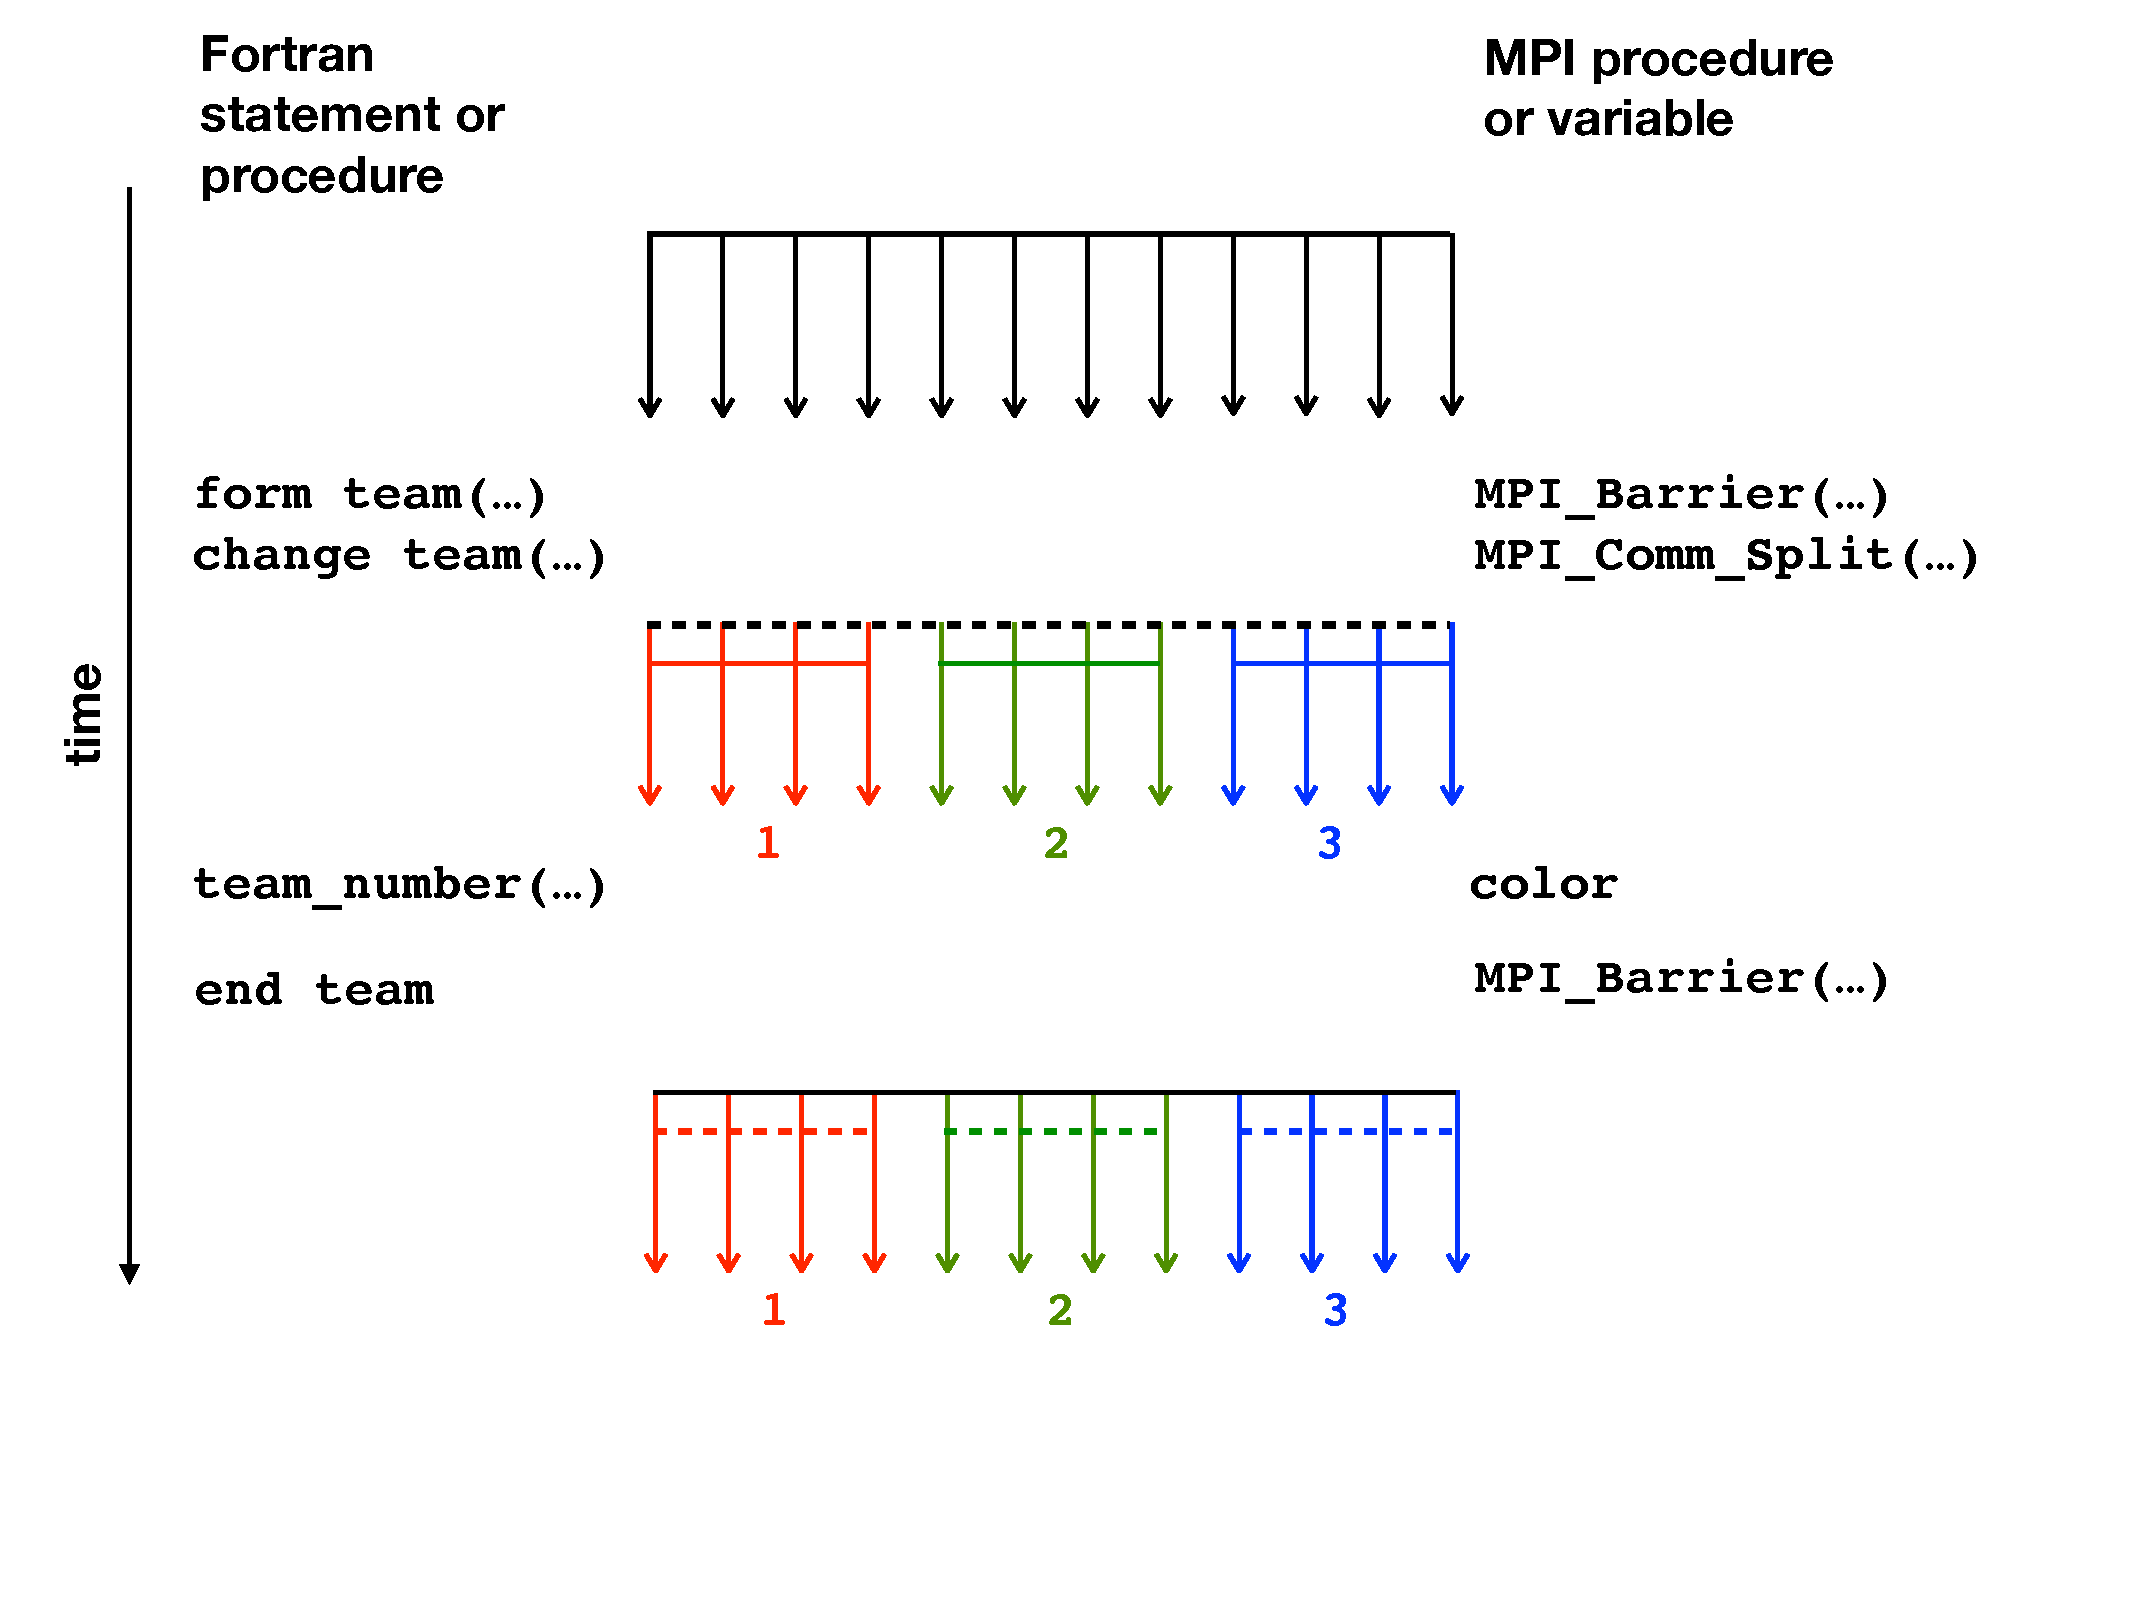
\includegraphics[width=0.7\textwidth]{figures/teams}
\vspace{-36pt}
\caption{Schematic depiction of a Fortran program executing over time (left axis) in 12 images (top) thatcommunicate with each other through global means (black horizontal bar) and later communicating within subgroups (colored horizontal bars).  Horizontal lines represent the communication mechanisms (default=solid, optional=dashed).  Fortran concepts or on the left.  The underlying \gls{mpi} concepts are the right.}
\end{figure*}
%

\begin{figure*}
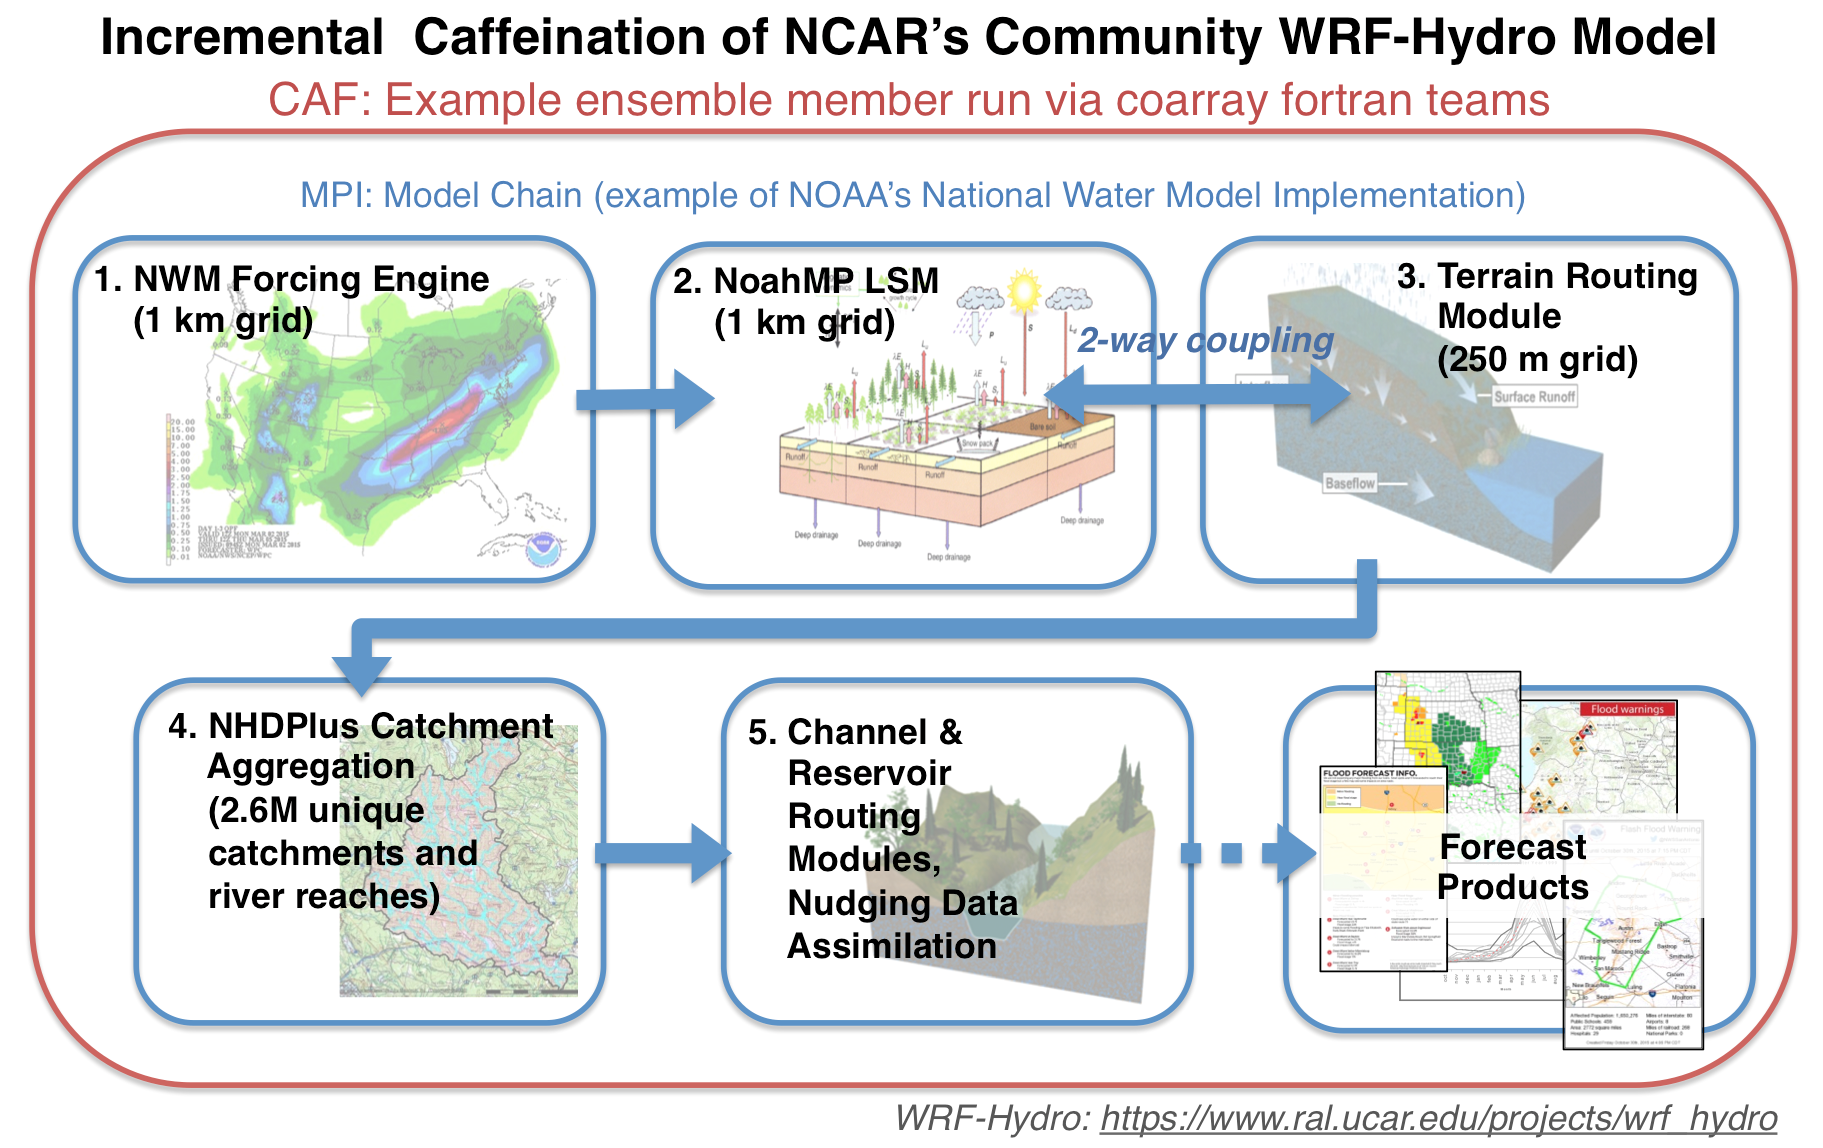
\includegraphics[width=0.7\textwidth]{figures/WRF-Hydro-caf-ens-model_chain.png}
\vspace{-7pt}
\caption{Example showing the partially caffeniated WRF-Hydro Model Chain (NOAA's National Water
  Model Implementation) which is already under MPI (in blue = decaf). Coarray
  fortran teams are applied to multiple model chains as ensemble members under the same
  executable. One such ensemble member is shown in the red box.}
\end{figure*}
%

%%%
%%% Sample tables
%%%

%\begin{table}
%  \caption{Frequency of Special Characters}
%  \label{tab:freq}
%  \begin{tabular}{ccl}
%    \toprule
%    Non-English or Math&Frequency&Comments\\
%    \midrule
%    \O & 1 in 1,000& For Swedish names\\
%    $\pi$ & 1 in 5& Common in math\\
%    \$ & 4 in 5 & Used in business\\
%    $\Psi^2_1$ & 1 in 40,000& Unexplained usage\\
%  \bottomrule
%\end{tabular}
%\end{table}

%\begin{table*}
%  \caption{Some Typical Commands}
%  \label{tab:commands}
%  \begin{tabular}{ccl}
%    \toprule
%    Command &A Number & Comments\\
%    \midrule
%    \texttt{{\char'134}author} & 100& Author \\
%    \texttt{{\char'134}table}& 300 & For tables\\
%    \texttt{{\char'134}table*}& 400& For wider tables\\
%    \bottomrule
%  \end{tabular}
%\end{table*}
% end the environment with {table*}, NOTE not {table}!

%It is strongly recommended to use the package booktabs~\cite{Fear05}
%and follow its main principles of typography with respect to tables:
%\begin{enumerate}
%\item Never, ever use vertical rules.
%\item Never use double rules.
%\end{enumerate}
%It is also a good idea not to overuse horizontal rules.


%%%
%%% Sample figures
%%%

%\begin{figure}
%\includegraphics{fly}
%\caption{A sample black and white graphic.}
%\end{figure}

%\begin{figure}
%\includegraphics[height=1in, width=1in]{fly}
%\caption{A sample black and white graphic
%that has been resized with the \texttt{includegraphics} command.}
%\end{figure}

%\begin{figure*}
%\includegraphics{flies}
%\caption{A sample black and white graphic
%that needs to span two columns of text.}
%\end{figure*}
%
%\begin{figure}
%\includegraphics[height=1in, width=1in]{rosette}
%\caption{A sample black and white graphic that has
%been resized with the \texttt{includegraphics} command.}
%\end{figure}

%\end{document}  % This is where a 'short' article might terminate



\appendix
%Appendix A
\section{Code listing}
% This next section command marks the start of
% Appendix B, and does not continue the present hierarchy
\section{Anything else?}

\begin{acks}
  The authors would like to thank the CISL and RAL Visitor Program

  The work is
  supported by the \grantsponsor{GSxxxxx}{National
  Science Foundation China}{http://dx.doi.org/zz.yyyyy/xxxxx} under Grant
  No.:~\grantnum{GSxxxxx}{yyyyyyy}

\end{acks}
